% To compile single chapters put a % symbol in front of "\comment" and "}%end of comment" below 
%    and take off the % symbol from "\end{document" at the bottom line. Undo before compiling
%    the complete thesis
%%Note: You can only use \section command, you are not allowed, per TTU Graduate School, use
%%\subsection command for ghigher level subheadings. At most level 2 subheadings are allowed.

\chapter{DASP Feature Classification and Results}
\label{DASP Device Classification Chapter}

\section[Learning Overview]{Learning Overview}

The DASP algorithms described in Chapter \ref{DASP Algorithm Development Chapter} were specifically developed to align, cluster, or otherwise group URE signal features in a 2-D image structure, with a goal of providing a method for the detection, characterization, and classification of devices based upon their conducted URE.  To ascertain the performance of the DASP algorithms, conducted URE was first collected from a variety of electronic devices, as outlined in Chapter \ref{URE Data Collection Chapter}, to provide a suitable data set for evaluation.  In Chapter \ref{DASP Feature Extraction Chapter} a suite of algorithms was developed to scale and highlight features of interest within DASP images and, in addition, a method for extracting statistical features was also presented.  A processing flow for feature generation was defined in Chapter \ref{Simulation and Testing Configuration} to enable 1-D feature vector evaluation through LDA and k-NN machine learners.  Finally, all DASP images were scaled and stored as TIFF image files to enable image classification through MATLAB\textsuperscript \textregistered 's CNN deep learning framework.

Before evaluation of the classification performance of the DASP derived features, an initial unsupervised clustering analysis was performed on the statistical based features in Section \ref{Device Clustering Analysis} to determine if the features were separable and to better understand and visualize the data.  The DASP algorithms were evaluated for their performance in a one-versus-all classification configuration using LDA and k-NN with statistical-based features and CNN with the stored TIFF images in Section \ref{Single Device Classification}.  Section \ref{Multiple Device Classification} provides an evaluation of the DASP transforms and associated learning algorithms applied to an all-versus-all classification configuration where multiple URE signals were present in the same capture.  Finally, Section \ref{Clutter Analysis} presents analysis of a trained CNN's ability to detect URE clutter and associate unknown devices with known devices based upon their URE signatures. 

\section[Statistical Feature Clustering Analysis]{Statistical Feature Clustering Analysis}
\label{Device Clustering Analysis}

An initial clustering analysis was performed on the statistical based feature vectors to confirm the separability of device classes.  The feature vector for each sample was formed by concatenating features from all image segments (including the whole image) of all DASP transforms.  In the process of forming the feature vectors it was found that the MASP-Low Scatter, MASP-Low Edge Array, MASP-Low Radon Array, and MASP-High Scatter based statistical feature vectors contained invalid values.  Upon further examination, the scaling process applied to these DASP transforms resulted in a large number of columns and rows with all zeros and therefore generated undefined statistical values.  After removal of the four ill-formed DASP transform statistical feature vectors, the concatenation of the remaining feature vectors resulted in a combined feature matrix, $\textit{\bf{X}}_C$, of $12000$ samples by $1173$ features.  The $12000$ samples were the result of $1200$ samples per device with $9$ devices plus the \textit{None} class.  The $1173$ features were comprised of $13 \times 90$ features for the remaining $13$ DASP transforms plus the $3$ SCAP auto-covariance statistical features.

A Principal Component Analysis (PCA) rank reduction was applied to $\textit{\bf{X}}_C$ to reduce the feature space down to $3$ features, $\textit{\bf{X}}_{C,3}$, to aid in visualization.  Figure \ref{fig:cluster_truth} provides a 2-D scatter plot of the rank reduced statistical feature matrix with the class values encoded in the scatter colors.  With only $2$ features shown it was evident that at least $4$ classes (\textit{fluorescentlights}, \textit{dellmonitor}, \textit{dellxps}, and \textit{hpzbook}) were highly separable from the remaining $6$ classes.

\begin{figure}[tb]
	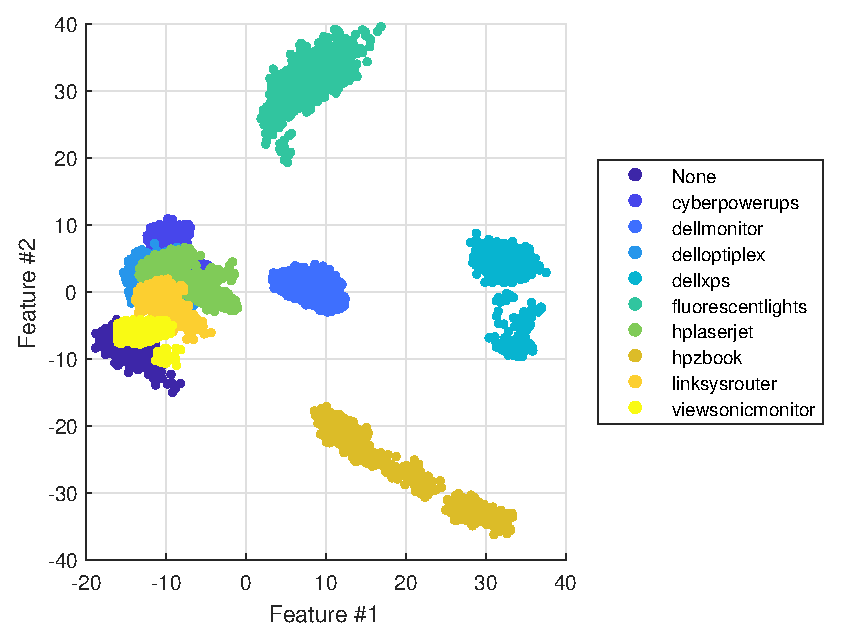
\includegraphics[width=\textwidth]{./dasp_algorithm_results/dasp_stat_cluster_truth.eps}
	\centering
	\caption{Scatter plot of the top two statistical features from the PCA reduced feature set.  The point colors represent the ground truth and show a clear separation among several of the classes (\textit{hpzbook}, \textit{dellxps}, \textit{fluorescentlights}, and \textit{dellmonitor}).}
	\label{fig:cluster_truth}
\end{figure}

Because only $4$ classes showed clear visual class separation through a 2-D projection of $\textit{\bf{X}}_{C,3}$, a gap analysis based upon a Gaussian-Mixture Model clustering was performed on the $\textit{\bf{X}}_{C,3}$ matrix to confirm the presence of approximately $10$ classes to further validate the data set.  Figure \ref{fig:cluster_gap} provides a plot of the gap values and corresponding standard deviations for $k = [1,2, \ldots, 19, 20]$\footnote{$k$ in the context of unsupervised clustering and k-means defines the number of classes (or clusters), as opposed to $k$ in the context of k-NN which corresponds to the number of nearest neighbors for supervised learning.}. 

\begin{figure}[tb]
	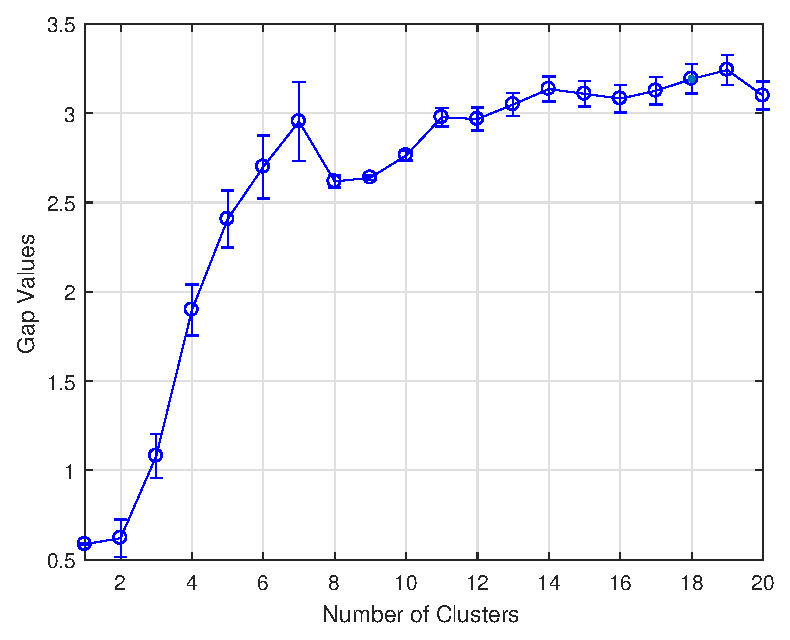
\includegraphics[width=\textwidth]{./dasp_algorithm_results/dasp_stat_cluster_gap.eps}
	\centering
	\caption{Plot of gap values with standard deviation error bars for the top three PCA reduced feature set, $\textit{\bf{X}}_{C,3}$.  The gap analysis shows a dip at $k=8$ with the minimum cluster variances between $k=8$ and $k=10$.}
	\label{fig:cluster_gap}
\end{figure}

Figure \ref{fig:cluster_gap} shows a dip in gap values at $k=8$ along with a corresponding drop in the standard deviation.  The minimum standard deviation occurs at $k=9$, with the second lowest standard deviation at $k=10$, which confirms the presence of approximately $8$ to $10$ classes.  Given that $k$ was known to be $10$, the gap assessment provided a good indicator that the statistical features were separable across all $10$ classes.  

A k-means clustering of the $\textit{\bf{X}}_{C,3}$ matrix with $k=10$ was then performed to further validate the results observed in the gap analysis, with the results shown in Figure \ref{fig:cluster_kmeans}.  The ``x'' marks show the k-means cluster centers, while the cluster colors are based upon a majority vote of known devices assigned to a particular cluster.  The k-means clustering did show many correct cluster assignments, however the \textit{hpzbook} cluster was incorrectly split in to two classes and the \textit{linksysrouter} class did not comprise the majority of any assigned cluster.

\begin{figure}[tb]
	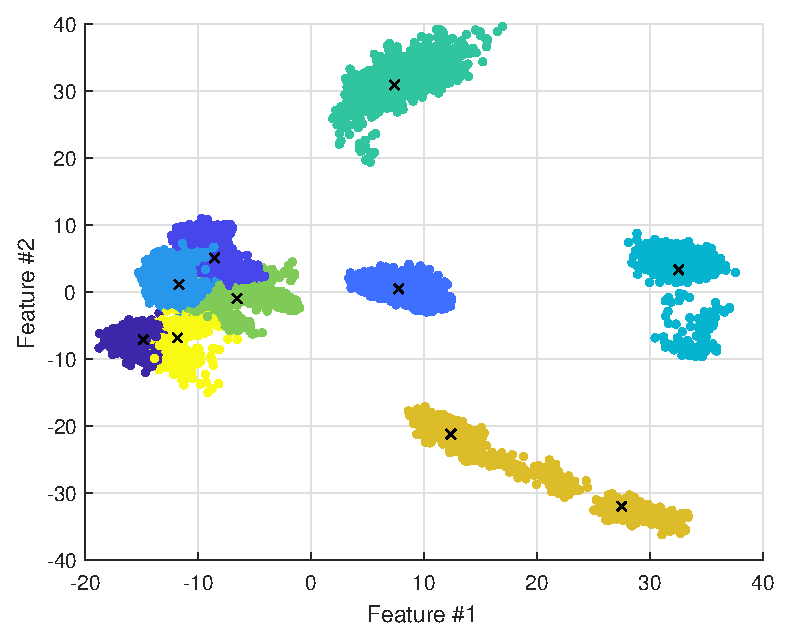
\includegraphics[width=\textwidth]{./dasp_algorithm_results/dasp_stat_cluster_kmeans.eps}
	\centering
	\caption{2-D scatter plot of a k-means clustering of top two statistical features from a PCA reduced feature set, with the ``x'' marks designating the k-means cluster centers.  The color coding and class assignments were based upon a majority vote of the known classes for a particular k-means cluster.  The k-means algorithm was not able to separate the \textit{linksysrouter} class from the overlapping clusters and incorrectly separated the \textit{hpzbook} class in to two separate clusters.}
	\label{fig:cluster_kmeans}
\end{figure}

Given the two distinct clusterings associated with the \textit{hpzbook} class, the k-means algorithm incorrectly separated the \textit{hpzbook} class and was therefore not able to generate a separate cluster with a majority of \textit{linksysrouter} devices.  The unsupervised clustering analysis showed that with only $3$ features the devices were mostly separable and indicated that a larger feature space may be required to correctly identify devices using supervised learning techniques.

\section[One-Versus-All Device Classification]{One-Versus-All Device Classification}
\label{Single Device Classification}

The DASP algorithms were first evaluated on their respective abilities to generate features relevant for one-versus-all classification.  Single device classification was performed based on the assumption that only one of the $10$ devices (or classes) was represented within a given sample.  One-versus-all classification was performed with LDA and k-NN learners on the statistical features as described in Section \ref{Statistical Features Single Device Classification}, whereas CNN learners were trained and tested against DASP images in a one-versus-all configuration as shown in Section \ref{Convolutional Neural Network Single Device Classification}.

\subsection[Statistical Feature Analysis]{Statistical Feature Analysis}
\label{Statistical Features Single Device Classification}

Before ascertaining the performance of the DASP-derived statistical features, several machine learning algorithms were evaluated based upon the following criteria:

\begin{itemize}
  \item Ability to provide one-versus-all multi-class classification results.
  \item Minimal or no “tuning” parameters.
	\item No prior knowledge of the class means or covariances.
	\item Robust and repeatable results.
	\item No requirement for an overly complex or optimum classifier.
	\item Retain some tie to the physical understanding of the underlying feature space.
	\item No requirement to handle class skew.
\end{itemize}
\label{list:ml_eval}

Several learning methods were explored for their applicability in evaluating the DASP statistical features, to include LDA, QDA, k-NN, Perceptrons, AdaBoost, and neural networks.  Although many of the candidate learning algorithms could have provided nearly optimum results in terms of classification, an optimized learner was not necessarily required for evaluation of the DASP-derived features.  Given the self-imposed requirements for the machine learning algorithm, neural networks and AdaBoost were eliminated based upon their high level of abstraction between the feature space and the learner, tuning parameter sensitivity, and repeatability \cite{Friedman2001}. 

The remaining algorithms, LDA, QDA, k-NN, and Perceptrons were further evaluated with LDA and k-NN eventually being utilized. Perceptrons may not converge or can take a long time to converge if the classes are not linearly separable and, in addition, the decision plane may change given different starting conditions \cite{Friedman2001}. LDA and QDA are closely related and differ only in the underlying assumption in the equality of class covariances with both providing similar classification performance.  LDA was eventually chosen for its simplicity, repeatability, and direct physical tie to the feature space where it attempts to maximize the distance between the class means and minimize the within-class variance \cite{Friedman2001}.  Certain assumptions were made about the underlying feature space for LDA to be a valid choice for classification.  LDA assumes that the feature means and variances are Gaussian distributed and each class shares the same covariance.  Furthermore, the utilization of LDA assumes that the classes are linearly separable. 

To balance the closed-form statistical-based solutions provided by LDA, k-NN was also used as an secondary learning method because of its non-parametric approach and simplicity.  In addition, k-NN does not make any assumptions about the underlying data such as linear separability and the equality of class covariances.  Although the choice of classifiers would have been re-evaluated had the early classification attempts performed poorly, LDA and k-NN were able to separate DASP generated statistical features at high classification accuracies ($>90\%$) in early testing and provided a robust and repeatable evaluation method for comparing the various DASP algorithms.

Table \ref{tab:stat_lda_acc} provides the results of a $4$-fold one-versus-all LDA classifier applied to the statistical-based DASP features for each of the $14$ DASP algorithm and image transform combinations as outlined in Table \ref{tab:dasp_config_parameters}, excluding the MASP-Low Scatter, MASP-Low Edge Array, MASP-Low Radon Array, and MASP-High Scatter combinations because of their previously noted invalid feature vectors.  Each DASP combination was evaluated using the entire feature set across all segments, $\textit{\bf{X}}$, using only the top image segment, $\textit{\bf{X}}_1$, and using a rank $3$ PCA reduced feature set.  The ``Combined'' DASP feature set, $\textit{\bf{X}}_C$, was formed by concatenating the $\textit{\bf{X}}$ feature vectors for all valid DASP algorithm and transform combinations.

\begin{table}[tb]
	\caption{One-versus-all 4-fold cross validation LDA classification accuracies for the statistically derived features.  All algorithms (except the SCAP-vec feature set) exceeded $95\%$ accuracy when all segments were used, while the majority still exceeded $82\%$ when only the top grid was leveraged.  }
	\csvautotabular{./dasp_algorithm_results/dasp_stat_lda_results.txt}
	\centering
	\label{tab:stat_lda_acc}
\end{table}

The results in Table \ref{tab:stat_lda_acc} show that using all segments, or $90$ features, provided accuracies exceeding $98\%$ for the majority of DASP combinations.  Using only $9$ features from the top segment provided accuracies on the order of $85\%$, with HASP-F Radon Array providing the highest accuracy at $94.7\%$.  The reduced rank feature sets performed worse, on average, than the $\textit{\bf{X}}$ and $\textit{\bf{X}}_1$ feature sets, however the rank reduced Combined feature set, $\textit{\bf{X}}_{C,3}$, was able to obtain an accuracy of $94.6\%$ with only $3$ features.  It should be noted that the although the combination of all segments and all feature sets, $\textit{\bf{X}}_C$, was able to reach an accuracy of $100\%$, it utilized a feature vector length of $1173$, or greater than $10$ times the number of features in the individual DASP combinations.

Table \ref{tab:stat_knn_acc} provides the results of a $4$-fold one-versus-all k-NN classifier applied to the statistical-based DASP features for each of the $14$ DASP algorithm and image transform combinations as outlined in Table \ref{tab:dasp_config_parameters}, excluding the MASP-Low Scatter, MASP-Low Edge Array, MASP-Low Radon Array, and MASP-High Scatter combinations.  The k-NN learner was configured to utilize an inverse-squared Euclidean distance metric with $k=10$ nearest neighbors.  Each DASP combination was evaluated using the entire feature set from all segments, $\textit{\bf{X}}$, only the top image segment, $\textit{\bf{X}}_1$, and using a rank $3$ PCA reduced feature set.  

\begin{table}[tb]
	\caption{One-versus-all 4-fold cross validation k-NN classification accuracies for the statistically derived features for all DASP algorithm and image transformations.  All algorithms (except the SCAP-vec feature set) exceeded $95\%$ accuracy when all grids were used, while the majority were in the $80\%$ range when only the top grid was leveraged.  Several of the PCA rank reduced feature sets exceeded $90\%$ with the combined feature set obtaining $96.7\%$, while the majority were in the $80\%$ range.}
	\csvautotabular{./dasp_algorithm_results/dasp_stat_knn_results.txt}
	\centering
	\label{tab:stat_knn_acc}
\end{table}

The results in Table \ref{tab:stat_knn_acc} show that using $\textit{\bf{X}}$, or $90$ features, provided accuracies exceeding $98\%$ for the majority of DASP combinations with the HASP-F Array, HASP-D Array, and Combined feature sets reaching $100\%$.  Using only $9$ features from the top segment, $\textit{\bf{X}}_1$, provided accuracies on the order of $95\%$, with the SCAP Array features providing the highest accuracy at $97.2\%$.  The reduced rank feature sets performed only slightly worse on average than the $\textit{\bf{X}}$ and $\textit{\bf{X}}_1$ feature sets, however the rank reduced Combined feature set, $\textit{\bf{X}}_{C,3}$, was able to obtain an accuracy of $97.2\%$, while the HASP-D Array, HASP-F Array, and FASP Array features sets also exceeded $90\%$ with only $3$ features.  As with the LDA results, it should be noted that although the $\textit{\bf{X}}_C$ feature set was able to reach an accuracy of $100\%$, it utilized a feature vector length of $1173$, or greater the $10$ times the number of features in the individual DASP combinations. 

The k-NN learning algorithm significantly outperformed the LDA learning method, especially with the Top segment and rank reduced feature sets indicating that the assumptions underlying the LDA algorithm, such as linear separability and Gaussian distribution of features, were not valid.  Figure \ref{fig:stat_cm_cum} provides a cumulative confusion matrix generated by averaging all of the confusion matrices of the LDA and k-NN learners.   

\begin{figure}[tb]
	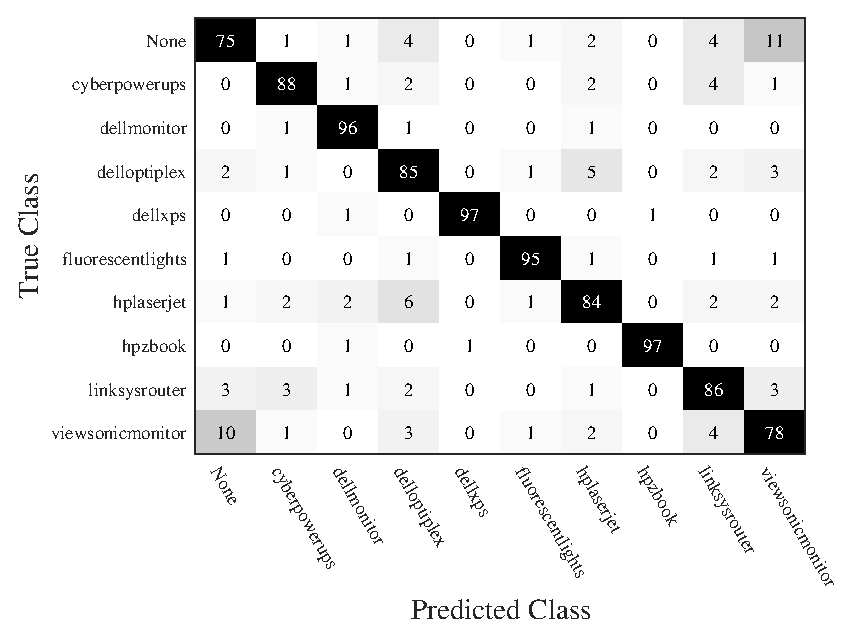
\includegraphics[width=\textwidth]{./dasp_algorithm_results/dasp_stat_AllCombined_conf.eps}
	\centering
	\caption{Cumulative confusion matrix for all of the results in Table \ref{tab:stat_lda_acc} and Table \ref{tab:stat_knn_acc}.  Results were obtained by summing the confusion matrices of all LDA and k-NN results and normalizing to percentages.  The table shows that the majority of the classes performed well with no strong confusion between two classes except for the \textit{viewsonicmonitor} class which was confused with the \textit{None} class at a rate of $11\%$.}
	\label{fig:stat_cm_cum}
\end{figure}

The cumulative results show that the largest confusion existed between the \textit{viewsonicmonitor} and \textit{None} devices with an $11\%$ misclassification rate.  The second highest misclassification rate of $6\%$ occurred between the \textit{delloptiplex} and \textit{hplaserjet} devices.  Interestingly, Figure \ref{fig:cluster_truth} shows significant overlap between the \textit{viewsonicmonitor} and \textit{None} classes and the \textit{delloptiplex} and \textit{hplaserjet} classes in the 2-D scatter plot of $\textit{\bf{X}}_{C,3}$, thus providing results consistent with Figure \ref{fig:stat_cm_cum}.

\subsection[DASP Image Analysis]{DASP Image Analysis}
\label{Convolutional Neural Network Single Device Classification}

Convolutional Neural Networks are a deep learning framework specifically designed for processing and classifying images and are widely used in the object recognition and computer vision communities.  CNNs have a variety of building blocks with an infinite number of configurations, but the foundational component of a CNN is the convolution (conv) layer.  The convolution layer is comprised of tunable filters that are updated through training to highlight areas, objects, or features within an image.  Convolution layers are typically followed by an activation layer and a pooling (pool) layer that ``scan'' and ``downsample'' the convolution filter outputs.  The pooling layer can ``downsample'' by several different methods, such as maximum pooling or averaging pooling, as it ``scans'' the convolution filter output by a fixed stride length.  The rectifying linear unit (reLU) implements the function $f(x) = \max(0,x)$ and is typically used as the activation layer.  A fully connected (fc) layer is implemented to connect with all input neurons and provide a scaled output by adding a bias and multiplying by a weighting factor.  The fully connected layer provides the higher level learning by calculating the appropriate convolution and pooling layer input weights for classification.   For instance, a series of convolution, activation, and pooling layers may learn an ``eye'', a ``nose'', and a ``mouth'', but the fully connected layer learns that together these features form a ``face''. 

As opposed to learning on feature vectors, as demonstrated in Section \ref{Statistical Features Single Device Classification}, a CNN trains and learns directly from the DASP images.  A very basic CNN was developed to perform one-versus-all classification of the DASP images, as described in Figure \ref{fig:cnn_net_single}.  The network consisted of an initial single-channel image input layer which resized the $500 \times 500$ pixel TIFF images to $25 \times 25$ pixels.  The input layer was followed by a convolution layer (\textit{conv1}) comprised of $20$ filters of size $5 \times 5$, a reLU layer, a max pooling layer (\textit{pool1}) with a $2 \times 2$ downsampling filter and a stride of $2$.  A fully connected layer (\textit{fc1}) with $10$ output neurons was utilized for the higher level learning.  A softmax classification layer was used to perform the one-versus-all classification.

\begin{figure}[htbp!]
	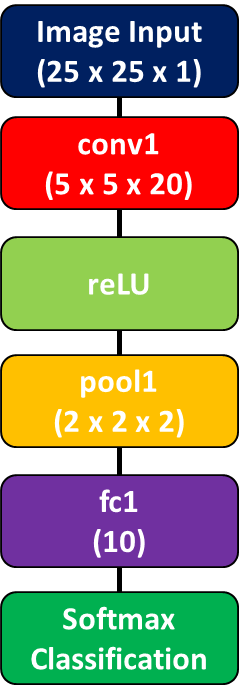
\includegraphics[width=0.3\textwidth,keepaspectratio]{./misc_graphics/dasp_cnn_simple_network.png}
	\centering
	\caption{Diagram of the Convolutional Neural Network used for one versus all device classification of DASP images. The network only utilizes one convolution, max pooling, and fully connected layer, in addition to a $25 \times 25$ image input layer.}
	\label{fig:cnn_net_single}
\end{figure}

The CNN in Figure \ref{fig:cnn_net_single} was trained using the parameters in Table \ref{tab:cnn_simple_train} where the Stochastic Gradient Descent with Momentum (SGDM) is defined by \footnote{https://www.mathworks.com/help/nnet/ref/trainingoptions.html, June $23$, $2017$}
\begin{equation}
    \theta_{l+1} = \theta_{l} - \alpha \nabla E \left(\theta_{l}\right) + \gamma \left( \theta_{l} - \theta_{l-1} \right)
		\label{eq:sgdmeq}
\end{equation}
where $l$ is the iteration number, $\alpha$ is the learning rate, $\theta$ specifies the updated parameter, and $E(\theta)$ is the cross entropy loss function
\begin{equation}
    E(\theta) = \sum^{n}_{i=1} \sum^{k}_{j=1} t_{ij} \ln y_{j} \left( x_{i},\theta \right)
		\label{eq:xentropyeq}
\end{equation}
 where $t_{ij}$ indicates the $i^{th}$ sample number is a member of the $j^{th}$ class and $y_{j}(x_{i},\theta)$ is the output for the $i^{th}$ sample.

\begin{table}[tb]
	\caption{Table of training parameters for the one-versus-all CNN.}
	\centering
		\begin{tabular}{c|c}
		\hline
		CNN Training Parameter & Parameter Value\\
		\hline
    Test Image Holdback Percentage & $20\%$ \\
		Learning Rate &  $1\times10^{-6}$\\
		Mini-Batch Size & $150$ \\
		Loss Function & Cross Entropy Function\\
		Update Algorithm & Stochastic Gradient Descent with Momentum\\
    \hline
		\end{tabular}
	\label{tab:cnn_simple_train}
\end{table}

Table \ref{tab:cnn_single_results} provides the blind testing results of the trained one-versus-all CNN.  All DASP image and transform combinations provided a greater than $97\%$ accuracy, with the SCAP Array being the best performer at $99.9\%$.  The MATLAB\textsuperscript \textregistered~CNN architecture does not allow for multiple column convolution streams\footnote{as of June, $2017$} so combined training on all DASP image combinations could not be implemented, but given the near optimal results from the individual DASP image transforms the combined training and testing was not required for the one-versus-all device classification.  

\begin{table}[tb]
	\caption{One-versus-all CNN classification results for all DASP algorithm processes.  All processes attained a greater than $97\%$ classification accuracy, with $10$ achieving accuracies greater than $99\%$.}
	\csvautotabular{./dasp_algorithm_results/dasp_cnn_results.txt}
	\centering
	\label{tab:cnn_single_results}
\end{table}

MATLAB\textsuperscript \textregistered ~ provides a method for inspecting a trained CNN network through the \textit{deepDreamImage} \footnote{https://www.mathworks.com/help/nnet/ref/deepdreamimage.html, July $06$, $2017$} command.  DeepDream image creation was developed by Google\textsuperscript \textregistered ~~ \cite{Mordvintsev2015} to allow researchers to visualize a composite image of layer activations within a trained network to develop understanding and insights into the learned features from a given training set.  Table \ref{tab:cnn_fc_dream_table} shows the \textit{deepDreamImage} outputs for the fully connected layers of select trained CNNs.  The DeepDream images looked very similar in structure to the DASP training images illustrated in Chapter \ref{DASP Algorithm Development Chapter} and Appendix B.  Appendix B provides sample images of all DASP transformations for all test and training devices in Table \ref{tab:collection_devices}.  The CMASP Edge Array DeepDream image, Figure \ref{fig:cnnfc2}, is particularly interesting in that a checkerboard pattern was formed to process the large number of intersecting lines and radials that are inherent to CMASP images.

{\centering
\begin{table}[tb]
	\caption{Table of DeepDream images of select fully connected layers from the one-versus-all CNNs trained on DASP images.  The DeepDream images highlight the learned activations associated with the DASP training images.}
	\begin{tabular}{ccc}
		\begin{subfigure}{0.3\textwidth}\centering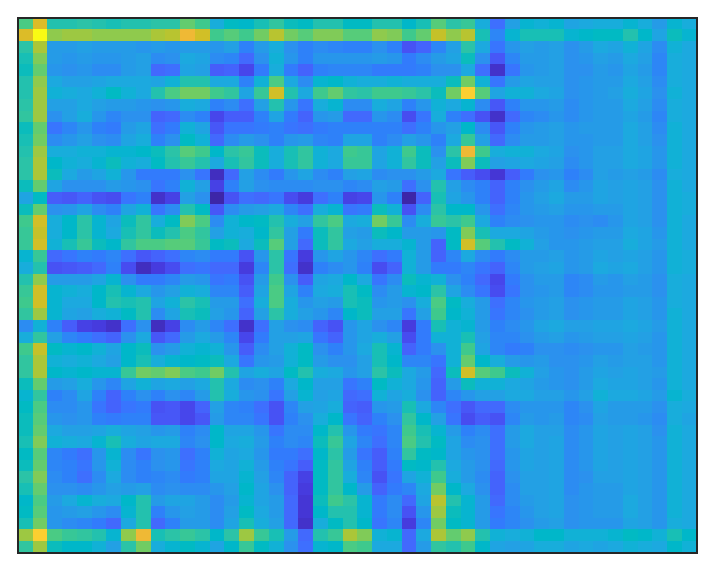
\includegraphics[width=0.8\columnwidth]{./dasp_algorithm_results/dasp_cnn_single_dream_fc_2.eps}
		\caption{CMASP, Edge Array}\label{fig:cnnfc2}
		\end{subfigure}&
		\begin{subfigure}{0.3\textwidth}\centering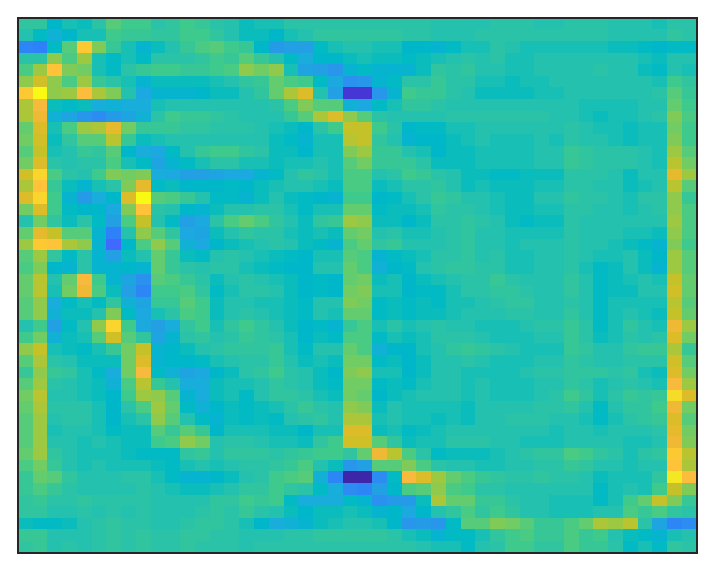
\includegraphics[width=0.8\columnwidth]{./dasp_algorithm_results/dasp_cnn_single_dream_fc_3.eps}
		\caption{CMASP, Radon Array}\label{fig:cnnfc3}
		\end{subfigure}&
		\begin{subfigure}{0.3\textwidth}\centering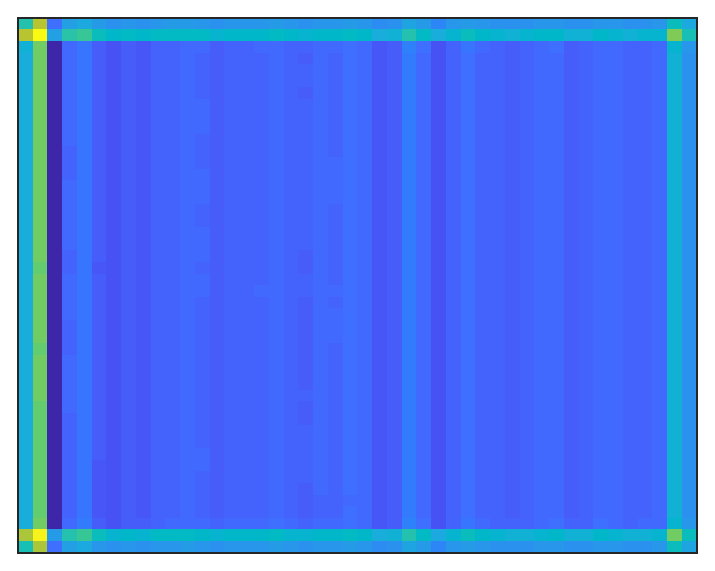
\includegraphics[width=0.8\columnwidth]{./dasp_algorithm_results/dasp_cnn_single_dream_fc_4.eps}
		\caption{FASP, Array}\label{fig:cnnfc4}
		\end{subfigure}    \\
		\begin{subfigure}{0.3\textwidth}\centering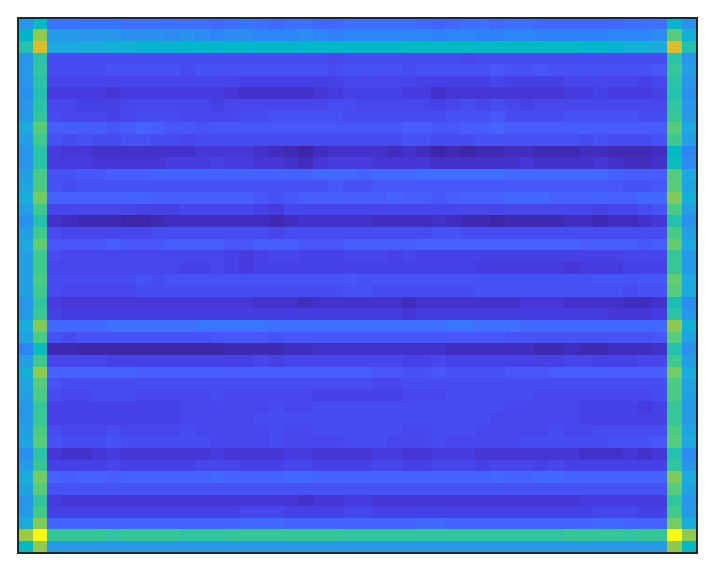
\includegraphics[width=0.8\columnwidth]{./dasp_algorithm_results/dasp_cnn_single_dream_fc_6.eps}
		\caption{HASP-F, Edge Array}\label{fig:cnnfc6}
		\end{subfigure}&
		\begin{subfigure}{0.3\textwidth}\centering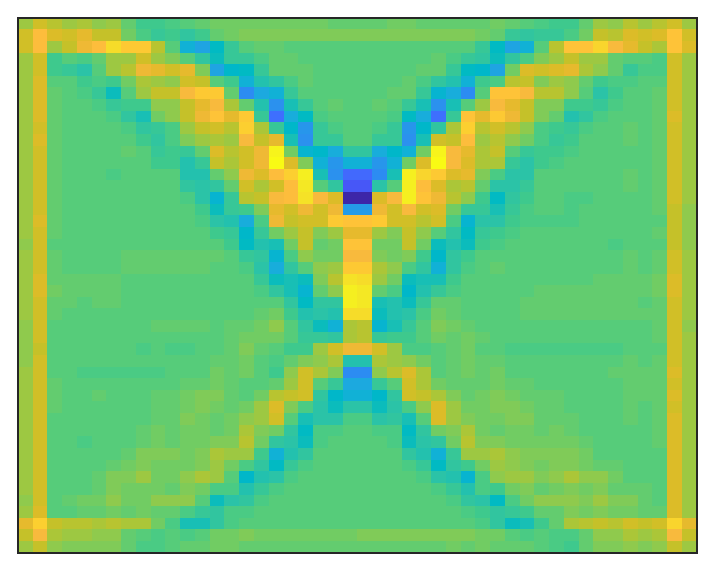
\includegraphics[width=0.8\columnwidth]{./dasp_algorithm_results/dasp_cnn_single_dream_fc_7.eps}
		\caption{HASP-F, Radon Array}\label{fig:cnnfc7}
		\end{subfigure}&
		\begin{subfigure}{0.3\textwidth}\centering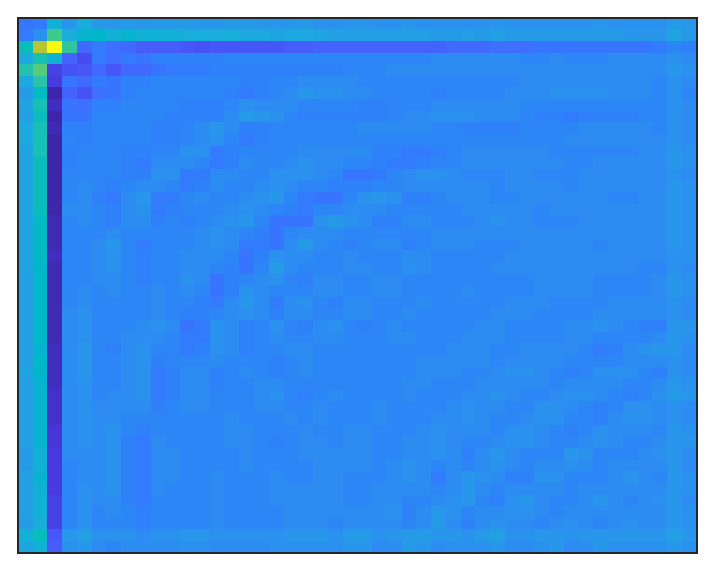
\includegraphics[width=0.8\columnwidth]{./dasp_algorithm_results/dasp_cnn_single_dream_fc_8.eps}
		\caption{HASP-D, Array}\label{fig:cnnfc8}
		\end{subfigure}    \\
		\begin{subfigure}{0.3\textwidth}\centering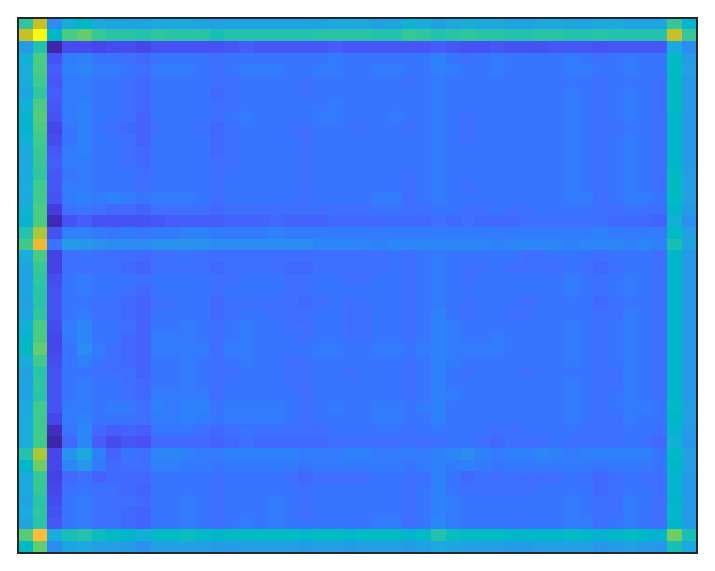
\includegraphics[width=0.8\columnwidth]{./dasp_algorithm_results/dasp_cnn_single_dream_fc_9.eps}
		\caption{MASP (Low), Array}\label{fig:cnnfc9}
		\end{subfigure}&
		\begin{subfigure}{0.3\textwidth}\centering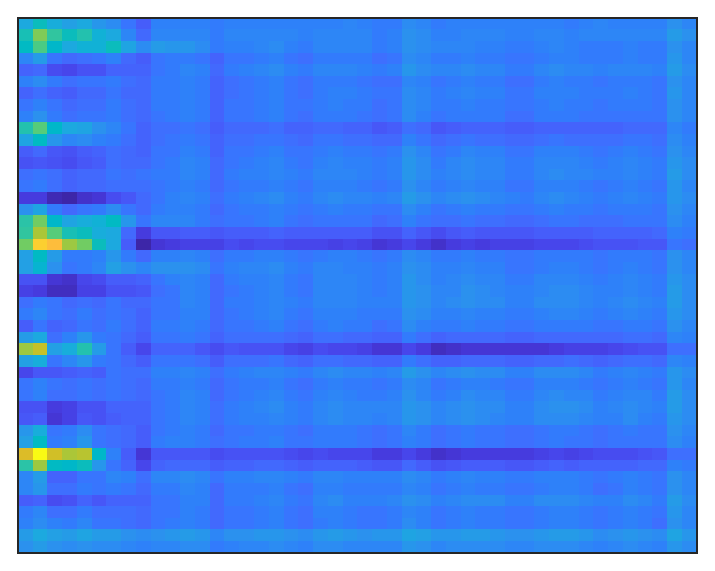
\includegraphics[width=0.8\columnwidth]{./dasp_algorithm_results/dasp_cnn_single_dream_fc_10.eps}
		\caption{MASP (Low), Scatter}\label{fig:cnnfc10}
		\end{subfigure}&
		\begin{subfigure}{0.3\textwidth}\centering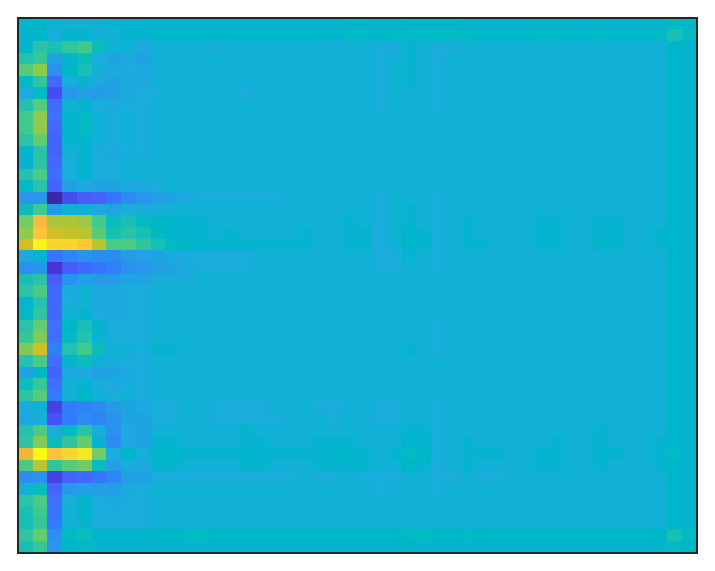
\includegraphics[width=0.8\columnwidth]{./dasp_algorithm_results/dasp_cnn_single_dream_fc_11.eps}
		\caption{MASP (Low), Edge Array}\label{fig:cnnfc11}
		\end{subfigure}    \\
		\begin{subfigure}{0.3\textwidth}\centering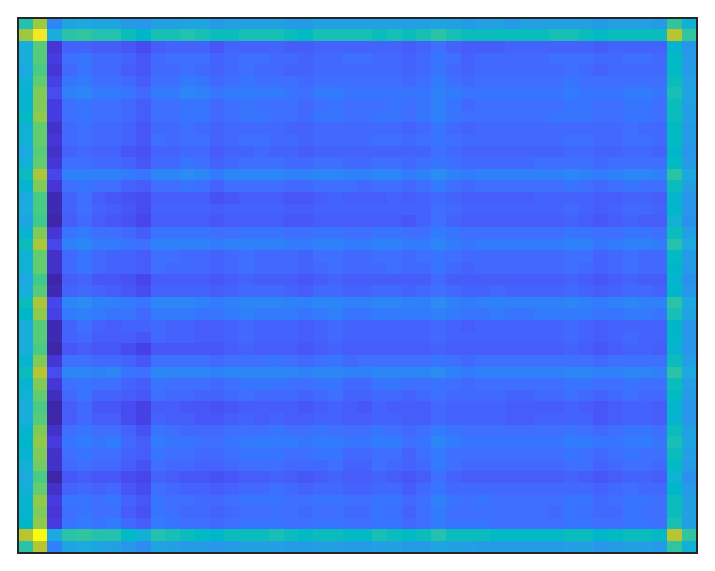
\includegraphics[width=0.8\columnwidth]{./dasp_algorithm_results/dasp_cnn_single_dream_fc_13.eps}
		\caption{MASP (High), Array}\label{fig:cnnfc13}
		\end{subfigure}&
		\begin{subfigure}{0.3\textwidth}\centering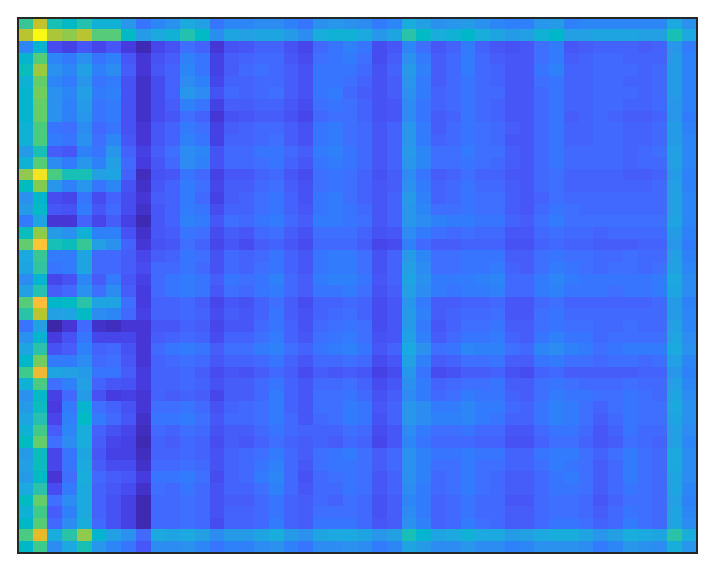
\includegraphics[width=0.8\columnwidth]{./dasp_algorithm_results/dasp_cnn_single_dream_fc_14.eps}
		\caption{MASP (High), Scatter}\label{fig:cnnfc14}
		\end{subfigure}&
		\begin{subfigure}{0.3\textwidth}\centering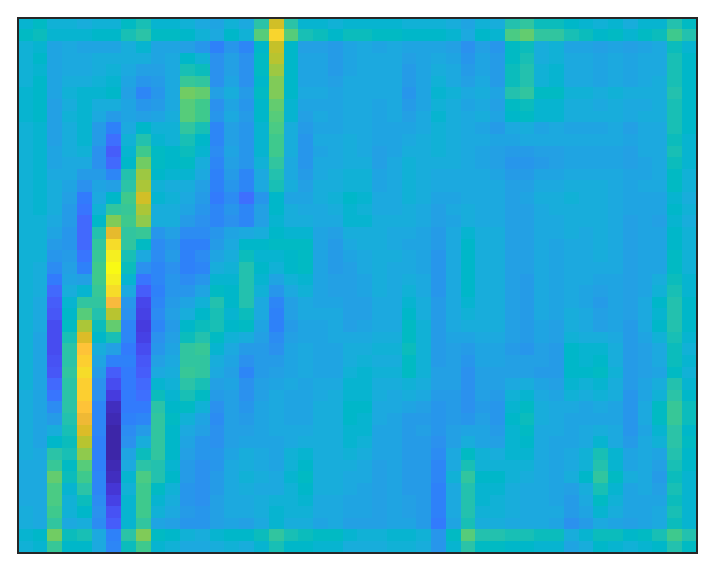
\includegraphics[width=0.8\columnwidth]{./dasp_algorithm_results/dasp_cnn_single_dream_fc_17.eps}
		\caption{SCAP, Array}\label{fig:cnnfc17}
		\end{subfigure}
	\end{tabular}
\label{tab:cnn_fc_dream_table}
\end{table}
}

\section[Multiple Device Classification]{Multiple Device Classification}
\label{Multiple Device Classification}

One-versus-all classification analysis in Section \ref{Single Device Classification} assumed that one and only one device was present in a given URE capture; however, that is not completely practical in an environment where many devices may be operating at the same time.  The LDA, k-NN, and CNN learners were all designed for one-versus-all classification and therefore were adapted for all-versus-all classification.  There are several methods for accomplishing multi-device detection and classification, 1) train a multi-class classifier for one-versus-all classification and set a threshold for detection, 2) train separate two-class classifiers for each device in a one-versus-none testing configuration, or 3) train a multi-class classifier with multiple labels per sample.  LDA cannot be trained as an all-versus-all multi-class classifier and therefore could not be easily adapted other than to develop a threshold for detection of present devices.  CNNs can be trained with multiple labels per sample given an appropriate network and loss function, however MATLAB\textsuperscript \textregistered ~ does not provide this functionality and therefore the CNN's previously trained on single-devices were adapted, similarly to the LDA learner, with a threshold to detect multiple classes.  \cite{Sorower2010, Zhang2007, Spyromitros2008} demonstrate the feasibility of using k-NN learners for multi-label classification, with the majority of the multi-label k-NN learners being adaptations of one-versus-none learning (Binary Relevance).  Given the threshold based approach of the LDA and CNN learners, the one-versus-all training of the LDA and CNN learners, and the redundancy in analyzing the statistical-based feature sets with k-NN, a multi-label k-NN was not utilized for processing of the multi-device statistical feature vectors. 

\subsection[Multiple Device Test Configuration]{Multiple Device Test Configuration}

Multi-device capture files were generated to test the single device trained LDA and CNN learners for multi-device classification.  The URE collection effort outlined in Chapter \ref{URE Data Collection Chapter} only collected a single device per capture, therefore single device captures were added in the time domain to form multi-device URE files.  One hundred multi-device captures were generated for each of $2$ through $9$ device combinations.  The multi-device combinations files were generated through a random selection process that excluded the \textit{None} state and more than one example of a class within a given multi-device file.  The multi-file generation process therefore generated $(9-2) \times 100 = 700$ multi-device test files.

The multi-device time domain files were subsequently processed with the DASP algorithms, feature extractors, and TIFF image creation processes outlined in Figure \ref{fig:dasp_lda_knn_process_flow} and Figure \ref{fig:dasp_cnn_process_flow}.  The generated multi-device DASP arrays and files were not used for training, but only as test inputs to the LDA and CNN learners trained on single devices.  To illustrate the superposition of multiple devices within a DASP image Figure \ref{fig:multi_device_image} shows the individual MASP (Low) scatter images for the \textit{cyberpowerups} and \textit{fluorescentlights}, as well as the combined MASP (Low) scatter image derived from the URE time domain superpositioning of the two devices.  The combined image shows artifacts of both the \textit{cyberpowerups} and \textit{fluorescentlights} device images as highlighted by the oval and circle, respectively.   

\begin{figure}[htbp!]
	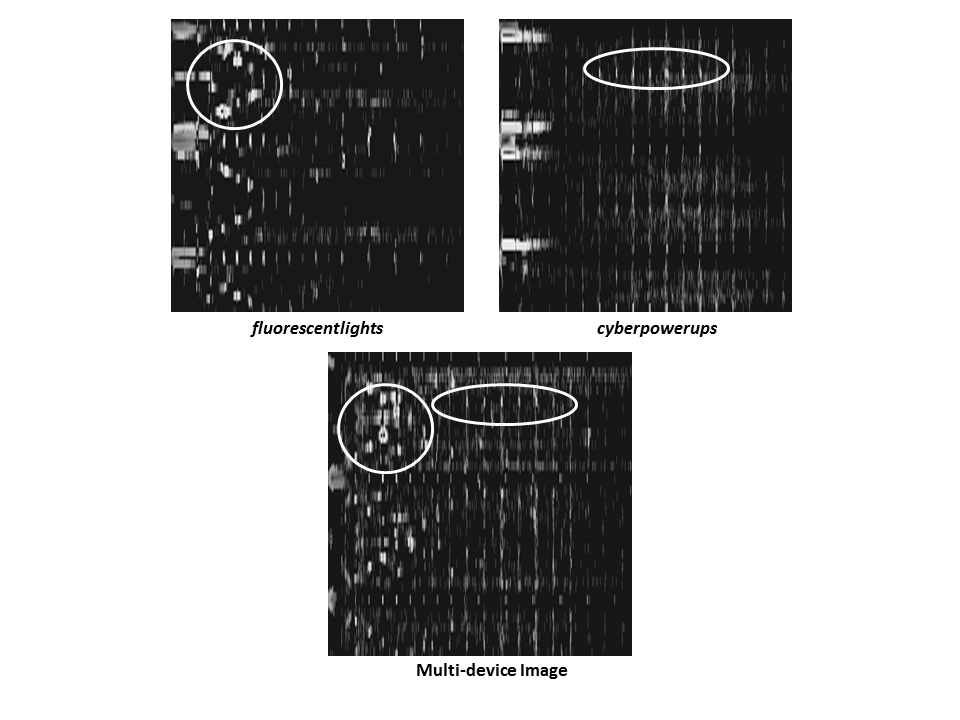
\includegraphics[width=\textwidth,height=\textheight,keepaspectratio]{./misc_graphics/multiDeivceImages.png}
	\centering
	\caption{MASP (Low) Scatter images for the \textit{cyberpowerups}, \textit{fluorescentlights}, and the multi-device combined image.  DASP image features for the \textit{cyberpowerups} and \textit{fluorescentlights} devices are shown by the oval and round circles, respectively.}
	\label{fig:multi_device_image}
\end{figure}

\subsection[Statistical Feature Analysis]{Statistical Feature Analysis}
\label{Statistical Features Multiple Device Classification}

The LDA learner trained in a one-versus-all method calculates a ``score'' for each class and selects the class with the greatest score.  To adapt for multi-device classification, the score vector was normalized using their z-score and a threshold of $0.5$ standard deviations was utilized to detect the presence of a specific class.  The results of the multi-device LDA classifier are shown in Table \ref{tab:stat_lda_multi} for each of the DASP combinations, including the results of the combined feature set.  The accuracy (ACC), true positive rate (TPR), false positive rate (FPR) true negative rate (TNR), false negative rate (FNR), precision (PR), and F-score (FSCORE) are provided. 

\begin{table}[tb]
	\caption{Classification accuracies and statistical measures of the multi-class LDA classifier using statistical based feature sets derived from all DASP algorithm processes.  Given $9$ possible class assignments with the \textit{None} class removed, the overall accuracies were around $50\%$.   Although the classifiers had significant False Negative Rates, the majority had Precisions exceeding $75\%$.  The MASP (High) Array feature set performed best with a precision of $1$, while only providing an accuracy of $50.9\%$ and a True Positive Rate of $0.2$.}
	\csvautotabular{./dasp_algorithm_results/dasp_stat_lda_all_multi_results.txt}
	\centering

	\label{tab:stat_lda_multi}
\end{table}

The results in Table \ref{tab:stat_lda_multi} show poor accuracy for all DASP combinations, however the false positive rates were relatively low which is further reflected in the high precisions, with the MASP (High) Array and Combined feature sets attaining precisions of $1$ and $0.96$, respectively.  Further analysis showed that the learners also had a high rate of false negatives, which taken in combination with the high precisions, means that while the LDA learners often missed the presence of a device they were detected with high confidence.  It should also be noted that the multi-device LDA learner was not trained on the \textit{None} state.  The assumption was made that the presence of a device was already determined and therefore the multi-device classifier was utilized to determine if a specific known device was present.

\subsection[DASP Image Analysis]{DASP Image Analysis}
\label{Convolutional Neural Network Multiple Device Classification}

The process of using a CNN learner trained on single devices to test for the presence of multiple device was handled in much the same way as that of the LDA learner in Section \ref{Statistical Features Multiple Device Classification}.  A score vector was extracted from the CNN network for each test sample and scaled by their z-score.  A threshold of $0.5$ standard deviations was then used to detect the presence of a given device.  To combine the DASP algorithms, the pre-normalized score vectors for each of the DASP algorithms were summed together, normalized, then compared to the detection threshold.  Early testing using the very basic CNN described in Figure \ref{fig:cnn_net_single}, showed very poor results due to network simplicity and over-training and, therefore, a new CNN was designed to better address multi-device classification and prevent over-training.

Figure \ref{fig:cnn_net_multi} shows the network topology of the multi-device CNN with reduced over-training susceptibility and improved multi-device classification performance.  The network used a single-channel image input layer that resizes input images to $100 \times 100$ pixels, as opposed to the $25 \times 25$ resolution in the single device CNN.  The input was connected to a $20\%$ dropout layer which was followed by two serially connected sets of convolution, reLU, max-pooling layers.  The dropout layer at the input sets each of its $100 \times 100$ pixel inputs to zero with a probability of $20\%$ to limit over-training of the network \cite{Srivastava2014}.  The two convolution layers, \textit{conv1} and \textit{conv2}, were each configured with $10$ filters of sizes $10 \times 10$ and $5 \times 5$, respectively. Both of the max-pooling layers utilized a $2 \times 2$ downsampling filter with a stride of one.  A fully connected layer (\textit{fc1}) with an output width of $100$ followed the convolution and pooling layers and feeds an additional reLU layer and $50\%$ dropout layer.  A final fully connected layer (\textit{fc2}) with an output width of $10$ was then followed by the softmax classification layer.  The dropout layers were added to specifically prevent, or at least limit, over training of the more complex network.  The additional convolution pooling layers were added to allow for processing of more complex shapes and structures within the DASP images, while the additional $100$ wide fully connected layer was included for higher levels of learning and abstraction.

\begin{figure}[htbp!]
	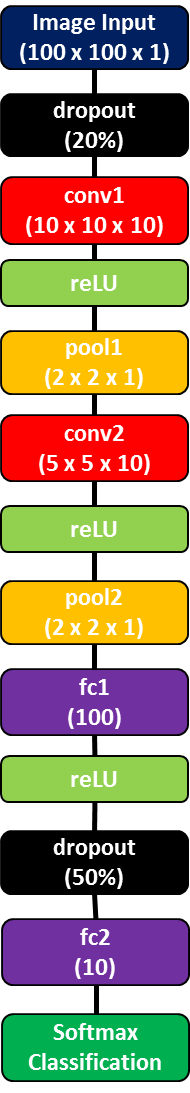
\includegraphics[width=0.2\textwidth,keepaspectratio]{./misc_graphics/dasp_cnn_multi_network.png}
	\centering
	\caption{Diagram of the Convolutional Neural Network used for multi-class device classification of DASP images. The input layer compressed input images to $100 \times 100$pixels, while only utilizing two convolution, max pooling, and fully connected layers along with two dropout layers to limit over training.  A fully connected layer of width $100$ was included to allow for higher level learning.}
	\label{fig:cnn_net_multi}
\end{figure}

The results from the multi-device testing of the trained multi-class CNNs are presented in Table \ref{tab:cnn_multi_testrmvd}.  The results for all $17$ of the DASP image and transform combinations is shown along with the combined CNN learner results.  Although the CNNs did not provide great accuracies, averaging slightly under $60\%$, they did outperform the LDA multi-device classifiers and were able to achieve a high average precision of $88\%$ with the combined results attaining a precision of $97\%$.  As with the LDA results, the CNN multi-device classifiers had high false negative rates, but reported the presence of devices with high confidence.

\begin{table}[tb]
	\caption{Classification accuracies and statistical metrics of the CNN multi-class classifiers.  The classification accuracies averaged around $60\%$, while classification Precisions were on the order of $0.90$. The combined CNN learner obtained an accuracy of $66.7\%$ and a $0.97$ precision.}
	\csvautotabular{./dasp_algorithm_results/dasp_cnn_multi_nonemultirmvd_results.txt}
	\centering
	\label{tab:cnn_multi_testrmvd}
\end{table}
 
Table \ref{tab:cnn_multi_acc_add_device} provides a listing of CNN multi-device classification results versus the number of devices present within a given test sample.  Initial inspection showed a monotonically decreasing accuracy which was to be expected in that more devices would result in more noise and signal confounders to contribute to misclassification, but for captures with less than $5$ devices accuracies exceeded $79\%$ with precisions exceeding $83\%$.  It should be noted that for $9$ devices in a given capture, there can be no false positives or true negatives in that all classes are present.  

\begin{table}[tb]
	\caption{Classification accuracies and statistical metrics of the CNN multi-class classifiers with respect to the number of devices within the test capture.  The relative accuracies monotonically decreased for each additional device, validating the testing approach.  The precisions monotonically increased ultimately reaching $1$ at $9$ devices, which was expected because all devices are present and any detected device was by definition the correct answer.}
	\csvautotabular{./dasp_algorithm_results/dasp_cnn_multi_nonemultirmvd_results_versus_numdevices.txt}
	\centering
	\label{tab:cnn_multi_acc_add_device}
\end{table}

In addition to analyzing the multi-class results based on the number of devices, an analysis was also performed to evaluate the classifier performance based upon the presence of a particular device type within a capture, with the results shown in Table \ref{tab:cnn_multi_acc_devtype}.  Several devices, \textit{dellxps}, \textit{fluorescentlights}, \textit{dellmonitor}, and \textit{hpzbook}, were more easily detected and therefore their presence and absence within a particular capture was determined with accuracies exceeding $80\%$, whereas the remaining devices had an average accuracy of $45\%$.  The precisions for all devices exceeded $90\%$, except for the \textit{viewsonicmonitor} which only had a precision of $62\%$.  The poor performance of the \textit{viewsonicmonitor} class was particularly noted in that it also showed significant confusion with the \textit{None} class in the cumulative confusion matrix in Figure \ref{fig:stat_cm_cum}.  

\begin{table}[tb]
	\caption{Classification performance of the CNN multi-class classifiers versus the presence of a given device type.  As shown, the \textit{fluorescentlights}, \textit{dellxps}, and \textit{hpzbook} specifically performed well with classification accuracies exceeding $98\%$ and precisions exceeding $0.97$.  The \textit{viewsonicmonitor} class was the least identifiable class with an accuracy of $39.8\%$ and a precision of $0.62$.}
	\csvautotabular{./dasp_algorithm_results/dasp_cnn_multi_nonemultirmvd_results_versus_devicetype.txt}
	\centering
	\label{tab:cnn_multi_acc_devtype}
\end{table}

Figure \ref{fig:cnnmultinonermvdroc} provides a Receiver Operation Characteristic (ROC) curve, along with the detection threshold utilized for the results in Tables \ref{tab:cnn_multi_testrmvd}, \ref{tab:cnn_multi_acc_add_device}, and \ref{tab:cnn_multi_acc_devtype}, for the combined multi-device CNN classifier.  The classifier was near perfect for the \textit{dellxps}, \textit{fluorescentlights}, and \textit{hpzbook} classes, with the next best classifier being for the \textit{dellmonitor}.  The remainder of the classifiers did not perform well with higher thresholds, which was confirmed by the high false negative rates observed in Table \ref{tab:cnn_multi_testrmvd} and Table \ref{tab:cnn_multi_acc_devtype}.  The \textit{viewsonicmonitor} classifier performed the worse and actually dips below the random guess boundary for higher thresholds as does the \textit{delloptiplex}.  A curve below the random guess line indicate that an increase in the threshold would result in a higher rate of false positives.  Because the ROC curves were generated for a multi-class classifier, a potential confounding feature from a different class may initiate a false positive output.  The detection threshold location indicated that a higher precision was attainable for the \textit{viewsonicmonitor} class with a lower threshold, however the false negative rates of several of the other device classes would have increased significantly.

\begin{figure}[htbp!]
	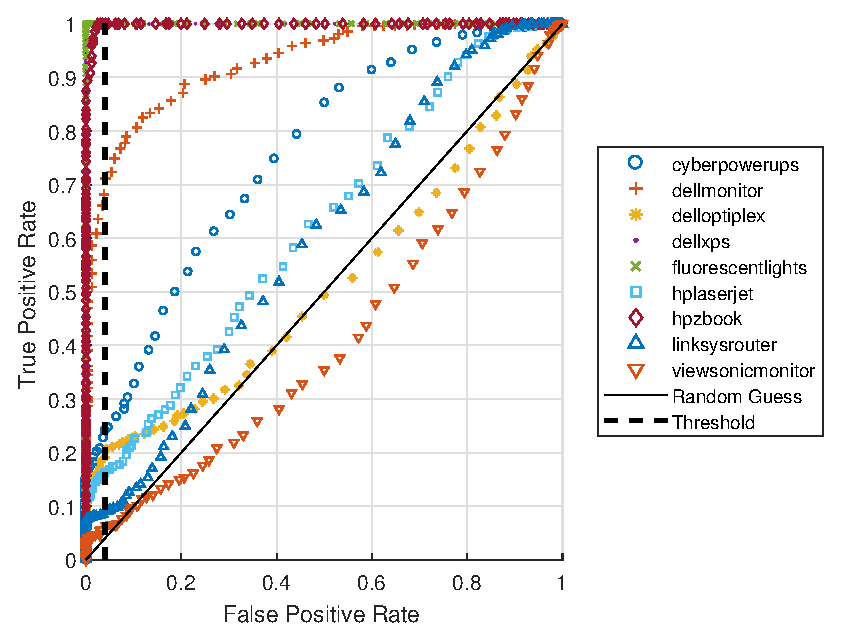
\includegraphics[width=\textwidth]{./dasp_algorithm_results/dasp_cnn_multi_nonemultirmvd_roc.eps}
	\centering
	\caption{Receiver Operation Characteristic curves for each class of the multi-class CNN classifiers.   As shown, two classes (\textit{viewsonicmonitor} and \textit{delloptiplex}) did not perform well with increasing thresholds and therefore seemed to be dominated by other class features at higher thresholds.  It was also shown that the \textit{hpzbook}, \textit{dellxps}, and \textit{fluorescentlights} obtained nearly perfect ROC curves with the multi-class CNN classifiers.}
	\label{fig:cnnmultinonermvdroc}
\end{figure}

DeepDream images were generated for the MASP (Low) Scatter plot trained multi-class CNN learner, Table \ref{tab:cnn_net_layers_masplscatter}, to provide a visual inspection of the composite layer activations for the more complex multi-class CNN.  DeepDream images were provided for both of the convolution layers, \textit{conv1} and \textit{conv2}, and the wider fully connected layer, \textit{fc1}.  The convolution layers performed lower level learning to determine the optimal filters for extracting features of interest from the DASP images, while the fully connected layer learned how to group these learned image features to identify specific devices.  As with the DeepDream images in Table \ref{tab:cnn_fc_dream_table}, each layer closely resembled the underlying structure of the input MASP (Low) images as presented in Section \ref{Modulation Aligned Signal Projection}.

{\centering
\begin{table}[tb]
	\caption{DeepDream images of the convolution layers and the first fully connected layer for the MASP (Low) Scatter plot multi-class CNN classifier.}
	\begin{tabular}{cc}
		\begin{subfigure}{0.5\textwidth}\centering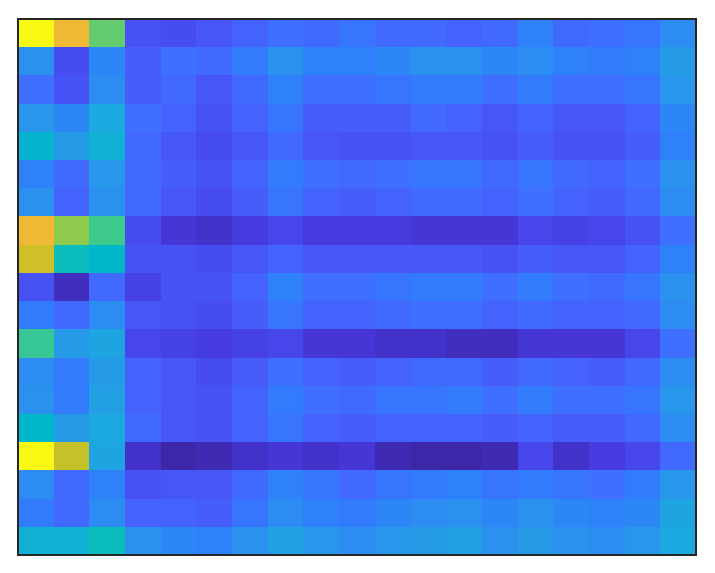
\includegraphics[width=0.9\columnwidth]{./dasp_algorithm_results/dasp_cnn_multi_nonermvd_dream_layers_3.eps}
		\caption{Convolution Layer \#1 (conv1)}\label{fig:cnnlayerconv1}
		\end{subfigure}&
		\begin{subfigure}{0.5\textwidth}\centering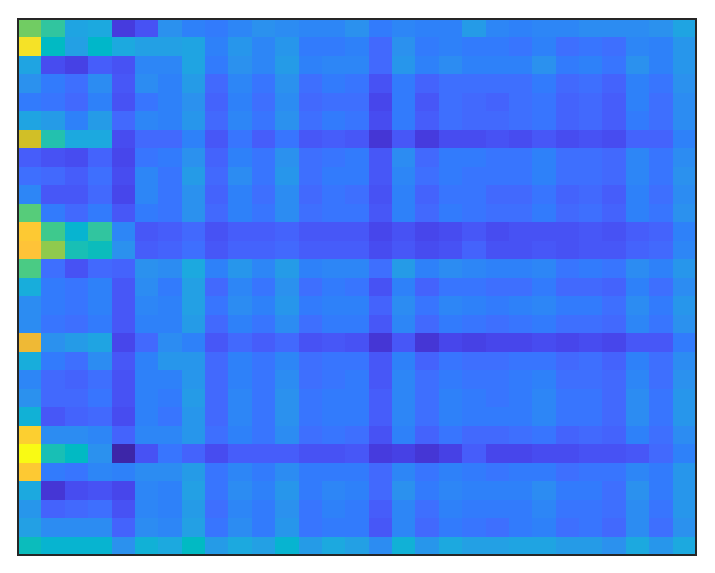
\includegraphics[width=0.9\columnwidth]{./dasp_algorithm_results/dasp_cnn_multi_nonermvd_dream_layers_6.eps}
		\caption{Convolution Layer \#2 (conv2)}\label{fig:cnnlayersconv2}
		\end{subfigure} \\
		\multicolumn{2}{c}{\begin{subfigure}{0.5\textwidth}\centering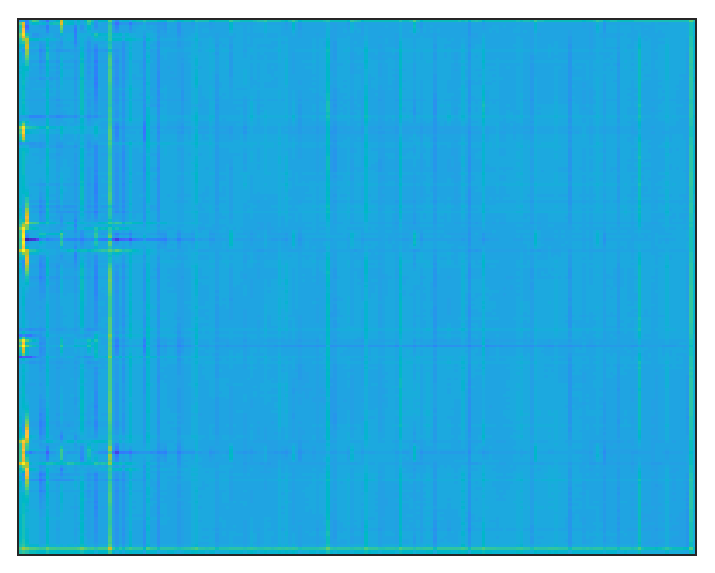
\includegraphics[width=0.9\columnwidth]{./dasp_algorithm_results/dasp_cnn_multi_nonermvd_dream_layers_9.eps}
		\caption{Fully Connected Layer \#1 (fc1)}\label{fig:cnnlayerfc1}
		\end{subfigure}}\\
	\end{tabular}
\label{tab:cnn_net_layers_masplscatter}
\end{table}
}

\section[Clutter Analysis]{Clutter Analysis}
\label{Clutter Analysis}

In addition to one-versus-all and all-versus-all multi-device classification, it was useful to understand the classifier response to URE clutter, or rather a device that had not been trained upon.  Clutter analysis was performed to 1) determine the ability of the classifier to ignore or otherwise not generate false positives when clutter is present and 2) develop a similarity measurement between a clutter input and known devices.  URE signal captures were performed on the clutter devices listed in Table \ref{tab:collection_devices} and processed with the same parameters and test conditions applied to the test device captures as described in Chapter \ref{Simulation and Testing Configuration}.  Analysis of the clutter URE DASP images was performed using the multi-class CNN as described in Section \ref{Convolutional Neural Network Multiple Device Classification}.  

The multi-class CNN classifier was presented with single clutter device DASP images and evaluated for the number of times the unknown device was misclassified as a previously observed device.  Table \ref{tab:cnn_clutter_percentage} provides the correct clutter assignment percentages for each of the DASP combinations.  A correct clutter assignment was defined as the clutter device not being classified as a known device.  Several of the DASP trained CNNs (FASP Array, HASP-D Array, MASP (Low) Array, and MASP (High) Array, performed very poorly and frequently misclassified a clutter device as a known device; however, the combination of DASP CNN classifiers was able to correctly identify clutter, or rather not identify as a known device, $80.9\%$ of the time.  The combined CNN testing was performed using a voting scheme between all of the trained CNNs and setting a fixed threshold for detection.   

\begin{table}[tb]
	\caption{Percentage of DASP clutter testing images that were correctly identified as \textit{clutter} for all DASP algorithm processes.   Although all of the algorithms performed poorly with only one providing a correct clutter identification over $50\%$ (MASP (Low) - Scatter), the combined vote across all algorithms provided an $80\%$ correct clutter assignment percentage.}
	\csvautotabular{./dasp_algorithm_results/dasp_cnn_clutter_percentage.txt}
	\centering
	\label{tab:cnn_clutter_percentage}
\end{table}

The results in Table \ref{tab:cnn_clutter_percentage} show that clutter devices presented to the trained CNNs resulted in a significant number of false positives.  To better understand the classes to which the clutter devices were incorrectly assigned and to understand the similarity between clutter devices and known devices, a confusion matrix was generated in Figure \ref{fig:cnn_clutter_percent} that outlines the percentage of ``likeness'' a clutter device was to a known device.   The ``likeness'' was determined by the cumulative score of each clutter device for each known class across all DASP combinations.  Each row provides the percentage that a given clutter device is similar to a known device, with each row summing to a full $100\%$. 

\begin{figure}[tb]
	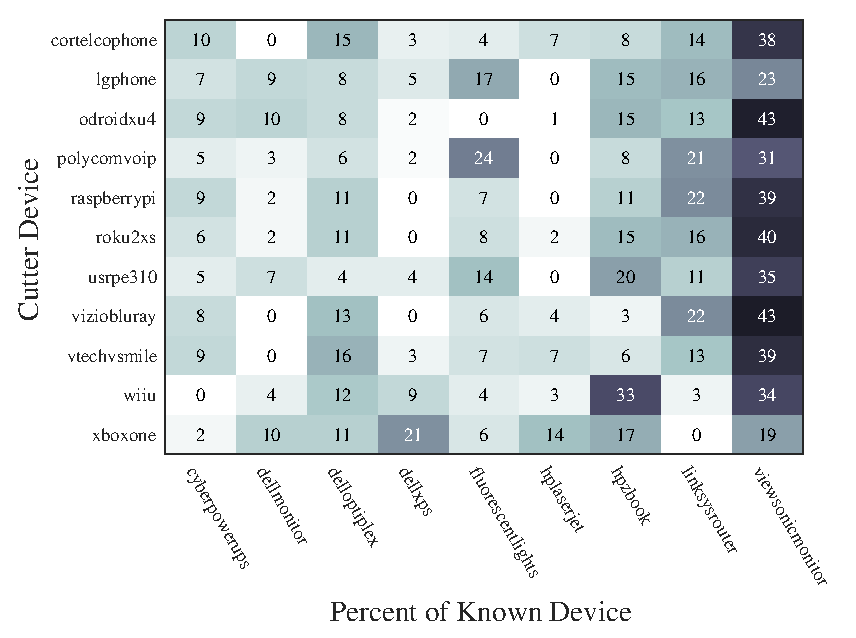
\includegraphics[width=\textwidth]{./dasp_algorithm_results/dasp_cnn_clutter_device_percentage.eps}
	\centering
	\caption{Confusion matrix showing the percentage similarity of each clutter device to previously trained devices.  Most devices have their strongest correlation with the \textit{viewsonicmonitor} on the order of $30\%$, with the \textit{linksysrouter} being the second most similar device on average.}
	\label{fig:cnn_clutter_percent}
\end{figure}

As with the previous results in Figure \ref{fig:stat_cm_cum} and Table \ref{tab:cnn_multi_acc_devtype}, the \textit{viewsonicmonitor} continued to confound several of the classifiers.  All of the clutter devices showed a strong and maximum resemblance to the \textit{viewsonicmonitor} device.   Given that the \textit{viewsonicmonitor} was most often confused with the \textit{None} class, as demonstrated in Figure \ref{fig:cluster_truth} and Figure \ref{fig:stat_cm_cum}, it was hypothesized that the similarity of the clutter devices to the \textit{None} class caused the strong response to the \textit{viewsonicmonitor} class.   Because all devices were collected with the same process and in the same environment, they all share certain vestiges of the underlying ``off'' state which possibly resulted in the high rate of \textit{viewsonicmonitor} misclassifications.

\section[Results Analysis]{Results Analysis}
\label{Results Analysis}

In Section \ref{Single Device Classification} the performance of features derived from the DASP algorithms was evaluated in a one-versus-all learner configuration.  Three different learners, LDA, k-NN, and CNN, were used to train and learn on statistical based features and DASP images.  Evaluation of the statistical based features with LDA and k-NN demonstrated the viability of DASP based features for device URE classification.  The performance of the k-NN learner far exceeded that of the LDA learner with respective average accuracies of $91.5\%$ versus $84.1\%$.  This was most likely due the fact that the features were not linearly separable and therefore assumptions underlying the application of LDA were not valid.  Even with the poor average performance of LDA, the PCA reduced feature set was still able to achieve an accuracy of $94\%$ with only $3$ features, whereas the k-NN learner was able to attain $97.2\%$.  The k-NN learner was able to achieve $98\%$ accuracy for $7$ of the DASP algorithms with only $90$ features and $10$ DASP transforms exceeded $98\%$ with only $9$ features.  Even with the success of the k-NN learner applied to the statistical feature sets, the CNN learner applied to the DASP images was able to achieve an average accuracy of $99\%$ with the simplest of CNN network topologies and an input image resolution of only $25 \times 25$ pixels.

Section \ref{Multiple Device Classification} explored the separability of the DASP generated features when multiple devices were present within the same test sample.  The LDA learner was utilized with a score threshold methodology to evaluate the presence or absence of a particular device within a test capture.  Evaluation of the DASP statistical features with multi-device samples did not achieve accuracies much greater than $50\%$, but was able to obtain an average precision of $80\%$.  The CNN was also tested against multi-device captures and the simple CNN used for single device classification was found to perform poorly during early testing.  A new CNN topology was developed to better handle multiple classes and limit over-training.  The new multi-device CNN also did not achieve accuracies much above $50\%$ and only had an average precision of $82\%$, but was able to achieve a precision of $97\%$ when all CNN learners were used in combination.  Determining the classification accuracy versus the number of devices within a capture showed that for $4$ or less devices in a capture an $80\%$ device classification accuracy was achievable.  The goal was to determine the separability of DASP features for multi-device classification problems and the combining of CNN learners showed promise and seemed a viable approach for application to multi-device classification problem sets.  It should also be noted that the testing was only performed on one second snippets of data and given the low false positive rates observed with the multi-device learners, it seems reasonable and practical to average multiple observations over time to improve the multi-device performance of the learners.

In Section \ref{Clutter Analysis} the responses of the multi-device CNN learners were evaluated when presented with previously unobserved devices (i.e. clutter).  The goal was to determine the DASP image trained CNN classifier sensitivity to clutter devices as well as to develop a method for determining the similarities between known and unknown devices.  Although the individual CNN learners were not able correctly identify clutter at an accuracy greater than $50\%$, the combination of learners was able to properly assign an unknown device to a clutter class with an accuracy exceeding $80\%$.   Additionally, evaluation of the clutter devices showed a strong similarity with the \textit{viewsonicmonitor} device, which was explainable by the strong confusion between the \textit{None} and \textit{viewsonicmonitor} classes, as identified in Figure \ref{fig:stat_cm_cum}.

The analysis in Sections \ref{Single Device Classification}, \ref{Multiple Device Classification}, and \ref{Clutter Analysis} all demonstrated the viability and applicability of using DASP algorithms to generate strong features for detection, characterization, and classification of devices based upon their URE.  Although the results were not always optimal, especially in the case of clutter identification, improvements in the learning and training processes could significantly improve the results.  The performance of CNN learners for classification of DASP images far exceeded the performance of the LDA and k-NN learners applied to statistically derived feature sets.  Both the single device and multi-device CNN topologies were fairly simple, as compared to AlexNet \cite{Krizhevsky2012} for instance, and significant improvements could be made to the CNN architecture to target DASP specific images.  Additionally, the training, testing, and learning processes were developed to evaluate DASP specific features and could be adapted and improved to better address operational concerns, such as multi-device and clutter assignment requirements.  For instance, more training on samples with multiple combinations of devices and clutter could significantly improve the ability to identify devices and in addition a separate CNN leaner could be trained for each known device in a one-versus-none configuration to find a specific device instead of comparing one-versus-all. 

Using the results from Sections \ref{Single Device Classification} and \ref{Multiple Device Classification} an evaluation was performed on all of the classification results for all of the DASP algorithms.  An average of all of the accuracies and precisions for all of the DASP learners was calculated, along with the standard deviation for each of the accuracy results.  The results are presented in order from best to worst in Table \ref{tab:dasp_ranking_nullsrmvd}.  Because of the indeterminate statistics associate with the MASP (Low) Scatter, Edge, and Radon arrays, the accuracy results could not be computed for the statistical feature-based learning algorithms and therefore were not included in Table \ref{tab:dasp_ranking_nullsrmvd}.  Given that the raw MASP arrays outperformed their transformed counterparts in Table \ref{tab:cnn_single_results}, the exclusion of the MASP transformed arrays did not affect the overall rankings. 

\begin{table}[tb]
	\caption{Ranking of the average accuracies and for all of the DASP classifiers, statistical feature based and CNN image analysis, with the removal of the MASP (Low) scatter, edge, and radon arrays.}
	\csvautotabular{./dasp_algorithm_results/dasp_transform_scores_rank_nullsrmvd.txt}
	\centering
	\label{tab:dasp_ranking_nullsrmvd}
\end{table}

Examination of the results in Table \ref{tab:dasp_ranking_nullsrmvd} showed that the unprocessed DASP arrays outperformed their transformed counterparts for all DASP algorithms, except for CMASP.  The range of average accuracies was only $8\%$ with no significant deviations in the average accuracy.  The top $6$ DASP rankings were all represented by a different DASP algorithm, with the SCAP array ranking $9^{th}$ directly behind two HASP-F transformed arrays.  The results show that continued processing and transformations of the DASP images is not necessary for classification purposes and therefore the raw arrays can be used in most circumstances, except for the CMASP algorithm which ranked best with the Edge Array transformation.

The DASP algorithm parameters were chosen heuristically and did not take in to account \textit{a priori} knowledge of a device's URE characteristics.  Optimization of the DASP parameters to specific devices or classes of devices could significantly improve the results in Sections \ref{Single Device Classification} and \ref{Multiple Device Classification} and could potentially change the ranking of DASP algorithms in Table \ref{tab:dasp_ranking_nullsrmvd}; however, the superior performance of the raw arrays over the transformed DASP arrays (i.e. Edge and Radon transforms) would likely be maintained.

%\begin{figure}[tb]
	%\csvautotabular{./dasp_algorithm_results/dasp_transform_scores_rank.txt}
	%\centering
	%\caption{Ranking of the average accuracies and precisions for all of the DASP algorithm process classifiers, statistical features and CNN analysis.  In addition, the standard deviation of the accuracies is also provided to indicate the applicability across multiple learning methods.  The MASP images adnd associated transforms dominate the results, but because of the statistical instabilities from the image scaling the MASP scatter, edge, and radon arrays were only evaluated with the CNN classifier and therefore skew the results.}
	%\label{fig:dasp_ranking}
%\end{figure}

%{\centering
%\begin{table}[tb]
	%\begin{tabular}{ccc}
		%\begin{subfigure}{0.3\textwidth}\centering\includegraphics[width=0.8\columnwidth]{./dasp_algorithm_results/dasp_cnn_multi_nonermvd_dream_fc_2.eps}
		%\caption{Figure A}\label{fig:cnnmultifc2}
		%\end{subfigure}&
		%\begin{subfigure}{0.3\textwidth}\centering\includegraphics[width=0.8\columnwidth]{./dasp_algorithm_results/dasp_cnn_multi_nonermvd_dream_fc_3.eps}
		%\caption{Figure A}\label{fig:cnnmultifc3}
		%\end{subfigure}&
		%\begin{subfigure}{0.3\textwidth}\centering\includegraphics[width=0.8\columnwidth]{./dasp_algorithm_results/dasp_cnn_multi_nonermvd_dream_fc_4.eps}
		%\caption{Figure B}\label{fig:cnnmultifc4}
		%\end{subfigure}    \\
		%\begin{subfigure}{0.3\textwidth}\centering\includegraphics[width=0.8\columnwidth]{./dasp_algorithm_results/dasp_cnn_multi_nonermvd_dream_fc_6.eps}
		%\caption{Figure A}\label{fig:cnnmultifc6}
		%\end{subfigure}&
		%\begin{subfigure}{0.3\textwidth}\centering\includegraphics[width=0.8\columnwidth]{./dasp_algorithm_results/dasp_cnn_multi_nonermvd_dream_fc_7.eps}
		%\caption{Figure A}\label{fig:cnnmultifc7}
		%\end{subfigure}&
		%\begin{subfigure}{0.3\textwidth}\centering\includegraphics[width=0.8\columnwidth]{./dasp_algorithm_results/dasp_cnn_multi_nonermvd_dream_fc_8.eps}
		%\caption{Figure B}\label{fig:cnnmultifc8}
		%\end{subfigure}    \\
		%\begin{subfigure}{0.3\textwidth}\centering\includegraphics[width=0.8\columnwidth]{./dasp_algorithm_results/dasp_cnn_multi_nonermvd_dream_fc_9.eps}
		%\caption{Figure A}\label{fig:cnnmultifc9}
		%\end{subfigure}&
		%\begin{subfigure}{0.3\textwidth}\centering\includegraphics[width=0.8\columnwidth]{./dasp_algorithm_results/dasp_cnn_multi_nonermvd_dream_fc_10.eps}
		%\caption{Figure A}\label{fig:cnnmultifc10}
		%\end{subfigure}&
		%\begin{subfigure}{0.3\textwidth}\centering\includegraphics[width=0.8\columnwidth]{./dasp_algorithm_results/dasp_cnn_multi_nonermvd_dream_fc_11.eps}
		%\caption{Figure B}\label{fig:cnnmultifc11}
		%\end{subfigure}    \\
		%\begin{subfigure}{0.3\textwidth}\centering\includegraphics[width=0.8\columnwidth]{./dasp_algorithm_results/dasp_cnn_multi_nonermvd_dream_fc_13.eps}
		%\caption{Figure C}\label{fig:cnnmultifc13}
		%\end{subfigure}&
		%\begin{subfigure}{0.3\textwidth}\centering\includegraphics[width=0.8\columnwidth]{./dasp_algorithm_results/dasp_cnn_multi_nonermvd_dream_fc_14.eps}
		%\caption{Figure A}\label{fig:cnnmultifc14}
		%\end{subfigure}&
		%\begin{subfigure}{0.3\textwidth}\centering\includegraphics[width=0.8\columnwidth]{./dasp_algorithm_results/dasp_cnn_multi_nonermvd_dream_fc_17.eps}
		%\caption{Figure A again}\label{fig:cnnmultifc17}
		%\end{subfigure}
	%\end{tabular}
%\caption{Table of Deep Dream images of fully connected layers of select DASP transforms from multi network training}
%\label{tab:cnnultifcdreamtable}
%\end{table}
%}
%\begin{figure}[tb]
	%\includegraphics[width=\textwidth]{./dasp_algorithm_results/dasp_stat_cluster_kmed.eps}
	%\centering
	%\caption{Clustering of top two PCA features using Kmed}
	%\label{fig:clustertruth}
%\end{figure}
%
%
%\subsection[Device Similarity]{Device Similarity}
%
%\blindtext[1]
%
%\begin{figure}[tb]
	%\includegraphics[width=\textwidth]{./dasp_algorithm_results/dasp_stat_cluster_link.eps}
	%\centering
	%\caption{Dendrogram using top three PCA features}
	%\label{fig:clusterdendrogram}
%\end{figure}

%\subsection[Image Similarity]{Image Similarity}
%
%\blindtext[1]
%
%\begin{figure}[tb]
	%\csvautotabular{./dasp_algorithm_results/dasp_ssim_acc_results.txt}
	%\centering
	%\caption{Table of classification accuracies for SSIM image classification.   The \textit{x12} column only uses $12$ images for testing against per class, whereas the \textit{x120} uses 120 images per class for comparison.   The results show a classification improvement for most DASP algorithm processes with an increase in the number of comparison images.  The combined results show a $99.2\%$ and $98.7\%$ classification accuracy for \textit{x12} and \textit{x120} respectively.   The combined classification accuracy was based on a class vote across all DASP algorithm processes.}
	%\label{fig:ssim_acc}
%\end{figure}
%
%\begin{figure}[tb]
	%\includegraphics[width=\textwidth]{./dasp_algorithm_results/dasp_ssim_120_120_conf.eps}
	%\centering
	%\caption{Confusion matrix for the \textit{x12} combined SSIM classifier.   The \textit{None} class is misclassified as a \textit{viewsonicmonitor} in $8\%$ of tests.}
	%\label{fig:ssim_120_cm}
%\end{figure}
%
%\begin{figure}[tb]
	%\includegraphics[width=\textwidth]{./dasp_algorithm_results/dasp_ssim_1200_1200_conf.eps}
	%\centering
	%\caption{Confusion matrix for the \textit{x12} combined SSIM classifier.   The \textit{None} class is misclassified as a \textit{viewsonicmonitor} in $11\%$ of tests and as a \textit{linksysrouter} in $3\%$ of tests.}
	%\label{fig:ssim_1200_cm}
%\end{figure}

%\subsection[Image Similarity]{Image Similarity}
%
%\blindtext[1]
%
%\begin{figure}[tb]
	%\csvautotabular{./dasp_algorithm_results/dasp_ssim_multi_results.txt}
	%\centering
	%\caption{Classification accuracies and statistical measures of the multi-class classifier using SSIM based feature sets derived from all DASP algorithm processes.  Given $9$ possible class assignments with the \textit{None} class removed, the overall accuracies were around $45\%$, with none of the SSIM classifier Precisions exceeding $0.65$.}
	%\label{fig:ssim_multi}
%\end{figure}

%\begin{figure}[tb]
	%\includegraphics[width=\textwidth,height=\textheight,keepaspectratio]{./dasp_algorithm_results/dasp_cnn_multi_nonemultirmvd_class_acc_numdevices.eps}
	%\centering
	%\caption{Plot of the multi-class CNN classification results as shown in \ref{fig:cnn_multi_acc_add_device}.  The monotonic decrease in accuracies with no major discontinuities confirms the viability of the testing methodology.}
	%\label{fig:cnn_multi_acc_dev_plot}
%\end{figure}

%\begin{figure}[tb]
	%\csvautotabular{./dasp_algorithm_results/dasp_cnn_multi_nonermvd_results.txt}
	%\centering
	%\caption{The classification accuracies and statistical metrics for the multi-class CNN classifier is provided, when all DASP images are used for training, regardless of their utilization and presence in the training set.  The results are comparable and in some respects are $1$ to $5$ percentage points lower than the results in \ref{fig:cnn_multi_testrmvd}.  The slightly poorer results could be the result of over training and a single device's features dominating other devices in certain multi-class combinations.}
	%\label{fig:cnn_multi_acc_alltrained}
%\end{figure}
